 What is Libgedathon?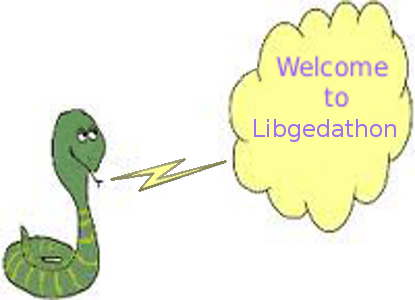
\includegraphics[scale=1]{./welcome_libgedathon.png} 

  Libgedathon is a extension library for LibgEDA that provides an intermediate API for Python. Libgedathon is not accessed directly. A seperate geda python extension module provides an interface to Libgedathon. The geda module provides a multi-level API as well as defining constants for use by Python programs. The API presented by Libgedathon allows creation and manipulation of gEDA objects for schematic and symbol files. The library does not manipulate data directly, per se, nor does the library perform any input or output operations. Libgedathon calls LibgEDA functions to perform operations on the data. Libgedathon does not currently provide any rendering capabilities or any API's for Libgedacairo. 
